\documentclass{article}
\usepackage{nips12submit_e,times}
\usepackage{textcomp}
\usepackage{graphicx}
\pagestyle{empty}
\nipsfinalcopy

\title{Zero-Shot Learning for Human Action Recognition}
\author{Nicole Rafidi \\
  \texttt{nrafidi@cs.cmu.edu}
  \And
  Yuzuko Nakamura \\
  \texttt{yuzi@cs.cmu.edu}
  \And
  Danny Zhu \\
  \texttt{dannyz@cs.cmu.edu}
}

\begin{document}
\maketitle

\begin{abstract}
We demonstrate the performance of zero-shot learning (ZSL) for the task of human action recognition from video. Instead of training a classifier to map from low-level video-extracted features directly to action labels, we instead define a set of semantic features using knowledge of human actions, and train regressors to map the videos to an intermediate semantic feature space, where each action label is a point in this feature space. We classify by choosing the canonical action point that is closest to the query point. This allows us to classify actions for which we have never seen video examples, a generalization that improves the feasibility of human action recognition. We demonstrate the efficacy of this technique with several experiments, and conduct a preliminary analysis of our semantic features.
\end{abstract}

\section{Introduction}
Zero-shot learning (ZSL) enables one to classify input with labels not seen in the training data. In other words, it allows a classifier learned on a limited data set to generalize to other labels. It does so by making use of a semantic knowledge base as an intermediate step between the features and classes \cite{Palatucci09}. The main objective of this project is to see whether zero-shot learning yields good performance in human action recognition, and enables us to classify actions that were never seen in training. Human action recognition is a domain in which there are many possible class labels (actions), making it intractable to provide examples of each action in a training set \cite{Poppe10}. This makes it a good candidate for improvement by zero-shot learning.

\section{Related Work}
Semantic knowledge bases, both user-defined (e.g. \cite{Vogel07} and \cite{Park04}) and automatically learned (e.g. \cite{Zhao10}), have previously been used as tools for learning and classifying actions. \cite{Vogel07} recognizes classes of outdoor scenes by segmenting an image into tiles and classifying each into a visual concept such as water, foliage, and rocks, and then using the resulting grids to perform classification. In order to describe motion, \cite{Park04} defines a set of operation triplets that each correspond to the way that specific body parts can move. A video sequence is translated into a subset of those triplets using domain-specific knowledge. Learning techniques using a bag of visual words approach to the problem such as \cite{Zhao10} often use algorithms to learn the semantics of a lower-level, raw visual vocabulary in order to achieve more accurate classification results.

Like our approach, these works all make use of an intermediate step to process low-level visual features into something more meaningful before performing classification. However, these approaches are only applied to the domain of training on a set of actions and classifying video containing those actions. By contrast, our approach makes use of a user-defined semantic knowledge base to enable a classifier to correctly classify actions not present in training data.

\section{Methods}
\subsection{Zero-Shot Learning}
Zero-Shot Learning is a form of two-stage learning. In the first stage, a mapping is learned from the training examples to the semantic space. These training examples may not contain examples of all possible labels. The second stage is a nearest neighbor classification - all labels (including those absent at training) are represented as points in the semantic space.  Classification is done by applying the learned regressor and then finding the closest label point in the semantic space.  Below we describe how we adapted this to the task of human action recognition.

We found a low-dimensional set of features to distinguish the labels (run, walk, etc). We designed the feature set based on our knowledge of human actions. A potentially better way to have selected this set would have been using text corpus statistics or surveys, but our feature set works reasonably well as a proof-of-concept. Thus, in our model, a 12-dimensional vector represents each action. These 12 features are discrete values corresponding to some canonical aspect of an action (e.g. `Is there horizontal displacement?'). See section \ref{sf} for the complete list of these features.

In the preprocessing stage, we extract low-level features from the videos using the spatio-temporal interest points algorithm, a 3-dimensional generalization of Harris points. The points are selected as the local maxima of a particular function on the video which selects for large local variation in all directions \cite{Laptev05}. We then compute an optical flow histogram (OFH) descriptor for each interest point. The x- and y-direction flow values in a neighborhood of a point are separately binned and the counts normalized. The two histograms are then concatenated to form the descriptor for each point. A single descriptor represents a whole video with a bag-of-features model. The OFH descriptors from all training videos are clustered by k-means, and any video then is represented by the normalized histogram of the clusters to which its OFH descriptors belong \cite{Laptev04}.

In the first stage of the classification process, 12 linear regressors are trained to map from the video features to the semantic features (one regressor per feature), using L2 regularized linear regression (CHECK). In the second stage, each action is represented by a point in this 12-dimensional feature space. To classify a video, the corresponding point is found, and the closest action point, by the Euclidean metric, is the label. See figure \ref{2stage} for a summary. While the semantic space is not necessarily Euclidean, using Euclidean distance works in practice.

\begin{figure}[h]
  \centering
  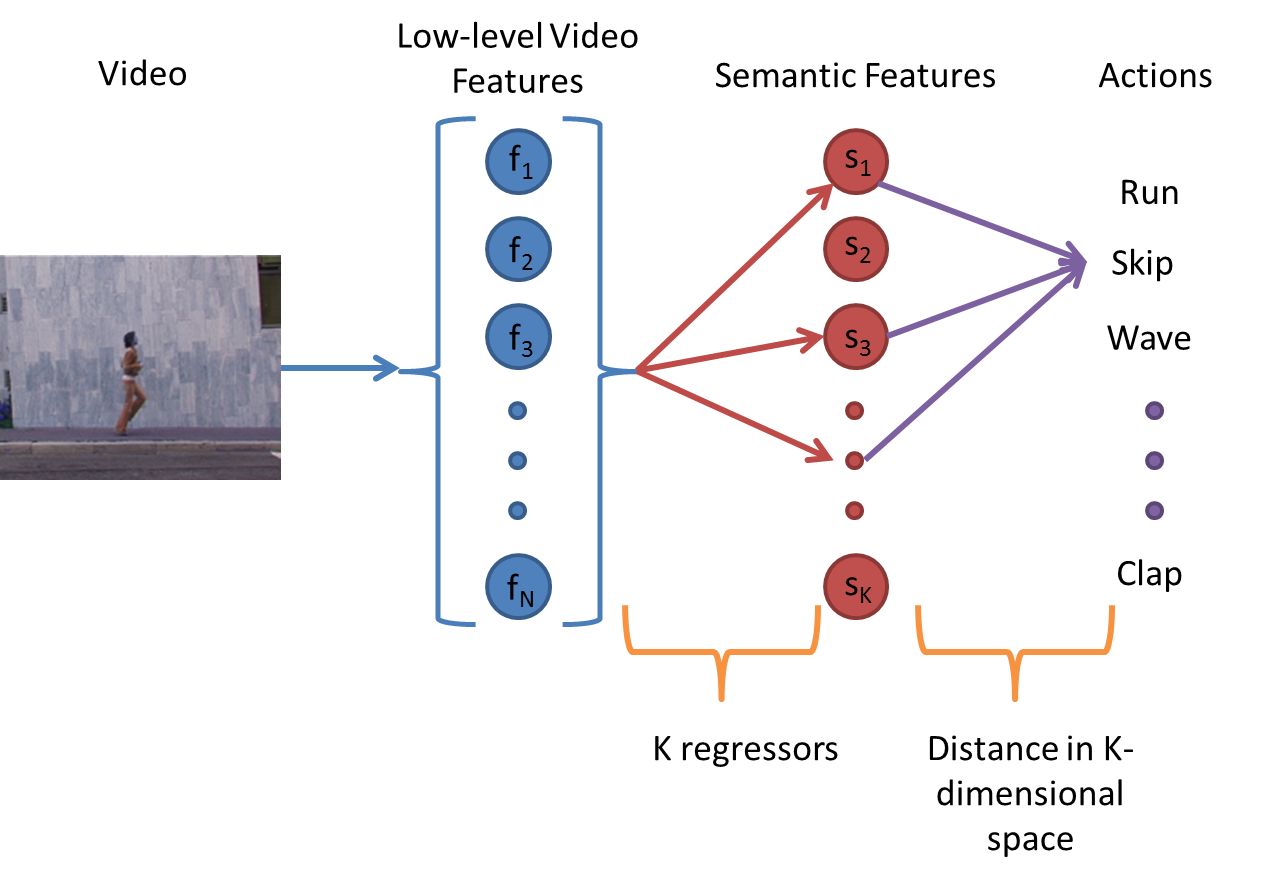
\includegraphics[width=.5\linewidth]{2stagelearning.png}
  \caption{A summary of the two-stage learning process. The low-level video features are optical flow hisogram descriptor clusters. We learn one regressors that map the low-level features to a dimension in the semantic feature space. Each action label is represented by a canonical point in that space.  To test a query point, we apply the regression and then perform nearest-neighbor classification in semantic space.}
  \label{2stage}
\end{figure}

\subsection{Leave-Two-Out Cross-Validation}
To test the effectiveness of this two-step method over direct video-to-label mappings, we can perform leave-two-out cross-validation, and demonstrate the ZSL classifier’s ability to distinguish between two previously unseen class labels based on their video data, a task that direct mappings are unable to perform.

First, the 12 regressors are trained on all but two of the actions. Then, a video of a previously unseen action is presented. This produces a query point in semantic space. The distance between the query point and the actual held-out action points is measured, and the point is classified. See figure \ref{ltocv} for a summary.

\begin{figure}[h]
  \centering
  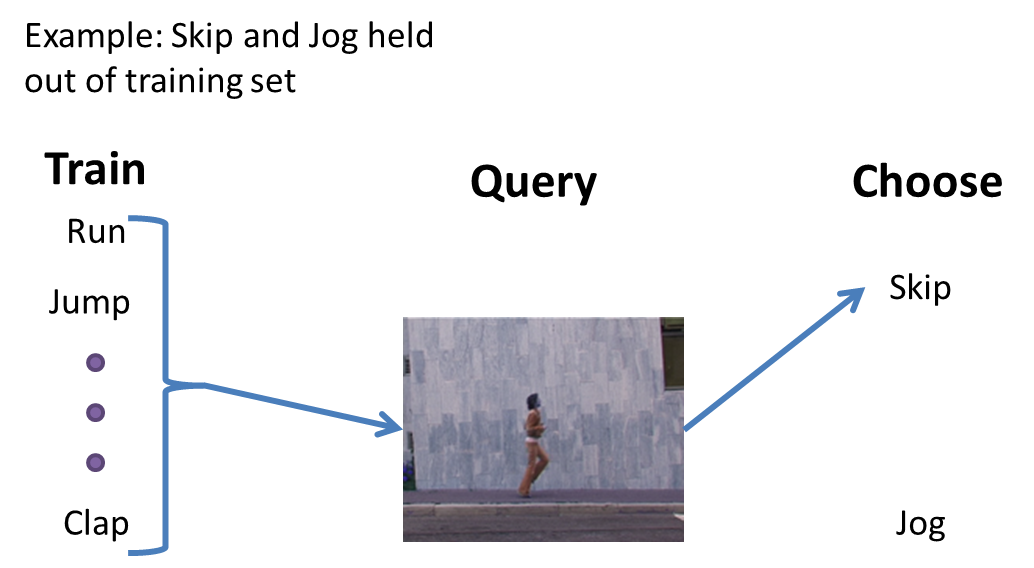
\includegraphics[width = .45\linewidth]{ltocv}
  \caption{A diagram summarizing the leave-two-out cross-validation used to test zero-shot-learning. The classifier is able to tell whether a video is of skipping or jogging, despite having never seen an example of either action. We rate performance on a per-action basis as the percent of videos correctly classified for every possible two vs two pairing for that action.}
  \label{ltocv}
\end{figure}

For each action label, we were able to produce a distribution of percent of videos correctly classified versus opposing action. So, the results have this structure (numbers invented for the sake of example):

\begin{table}[h]
\centering
\begin{tabular}{c|c|c|c|c}
Action/Action & Run & Walk & Wave & ... \\ \hline
Run & ---- & .70 & .90 & ... \\ \hline
Walk & .80 & ---- & .95 & ... \\ \hline
Wave & .90 & .99 & ---- & ... \\
\end{tabular}
\end{table}

This distribution can be compared to a simulated null distribution (described in Section \ref{stats}) to determine significance of the results via paired t-test.

\subsection{Rank Test}
A more difficult task than leave-two-out cross-validation would be to compare the query point to all possible points in the semantic space. This allows us to determine if the ZSL classifier is biased toward items it has seen during training. In this experiment, we held one action out during training, and then had the classifier output the rank of the true action label when given a query action. All actions, even those held out in training, are still present in the semantic space as points. We calculated from this a rank accuracy with the following equation:
\begin{equation}
accuracy = 1 - \frac{r}{T}
\end{equation}

Where $r$ is the rank of the true label and $T$ is the total number of action labels.  This can be thought of as a measurement of the percentage of the other labels that are ranked below the true label. A score of 1 is perfect (CHECK). The experiment is summarized in Figure \ref{ranking}.

\begin{figure}[h]
  \centering
  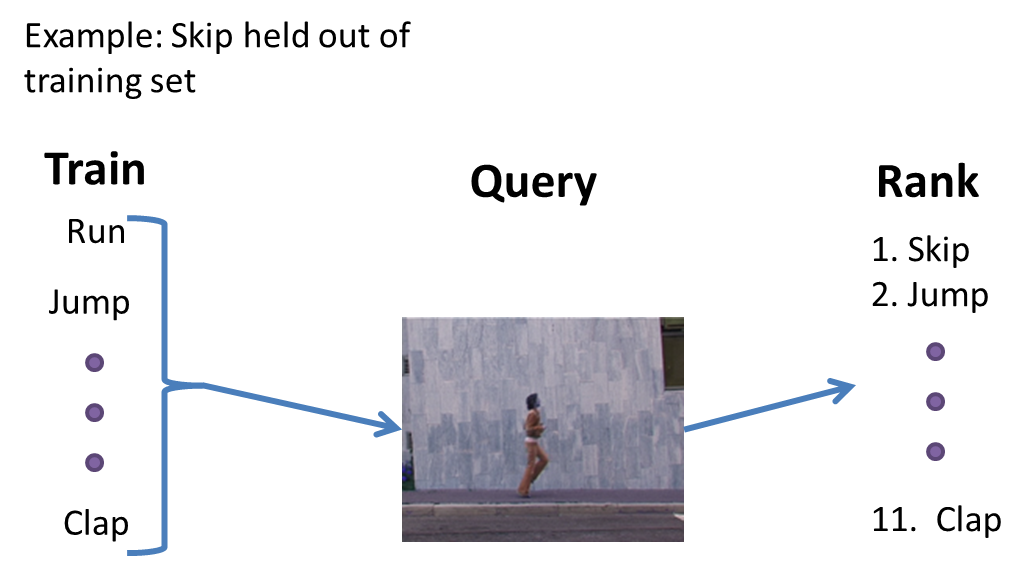
\includegraphics[width = .45\linewidth]{ranking}
  \caption{A diagram summarizing the rank test. The classifier ranks the potential action labels in order of nearness to the query point. Performance is measured with respect to the position of the true label.}
  \label{ranking}
\end{figure}
\label{rank}

For each held-out action, we calculated the rank accuracy of each video of that action. This created a distribution that we compared against a simulated null distribution (see Section \ref{stats} for details) for statistical significance.

\subsection{Feature Comparison}
To see which semantic features yield the biggest advantage in decoding the action, we can test the leave-two-out cross-validation performance using only a subset of the semantic features in the intermediate set. This wil allow us to see if particular features are stronger predictors than others.

In the first version of the experiment, we tried leaving each semantic feature out in turn and measuring the performance. See Figure \ref{feature} for an illustration.

\begin{figure}[h]
  \centering
  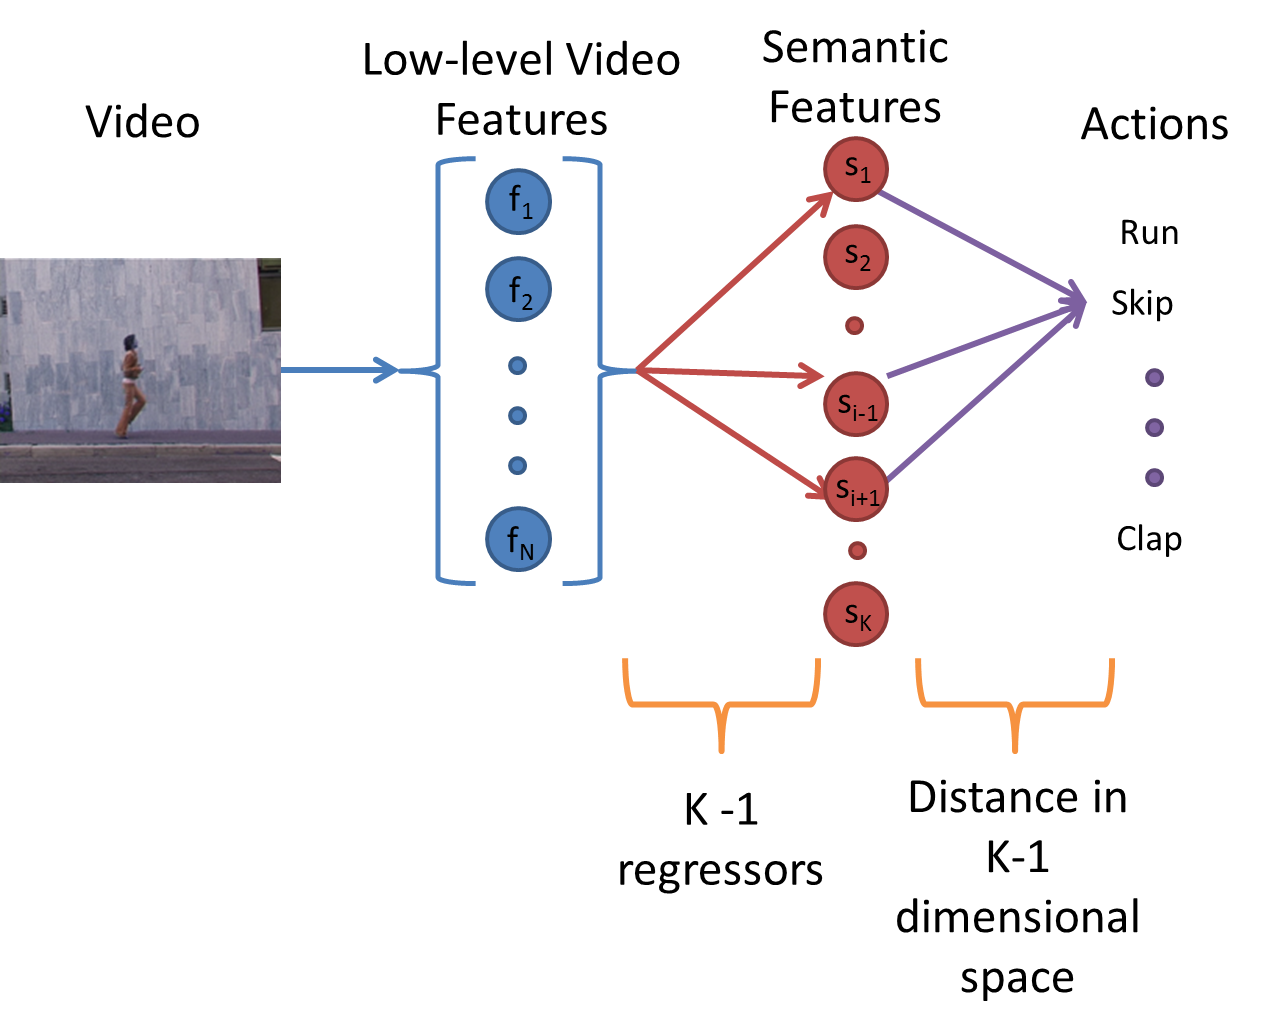
\includegraphics[width = .45\linewidth]{features}
  \caption{A diagram summarizing the feature comparison test. Each semantic feature was held out in turn and performance re-assessed using the method in Section \ref{ltocv}.}
  \label{feature}
\end{figure}

We also tried leaving out subsets of features that seemed highly correlated. We chose the following groups:

\begin{table}[h]
\centering
\begin{tabular}{c|c}
Feature Group & Features Contained\\ \hline
Coordination & Arm and leg coordination \\ \hline
Center of Mass & Torso motion and orientation, Horizontal and vertical displacement\\ \hline
Hand & Hand location \\ \hline
Speed & Speed of center of mass, and speed of each limb \\
\end{tabular}
\label{featgrp}
\caption{Semantic feature groups left out, and features contained in those groups.}
\end{table}

For each held out feature or group of features, we had a distribution of average leave-two-out cross-validation performance across actions.  We compared this to the distribution found when using all features.

\label{fcomp}

\subsection{Statistical Significance}
Each experiment generates a distribution of performance scores. The set of scores can be compared to chance with a paired t-test to establish significance.

We establish chance with a permutation test. We sever the connection between the videos and their semantic feature labels and shuffling the data. The semantic feature space points representing the acitons remained tied to their actions. See Figure \ref{st} for an illustration.

\begin{figure}[h]
  \centering
  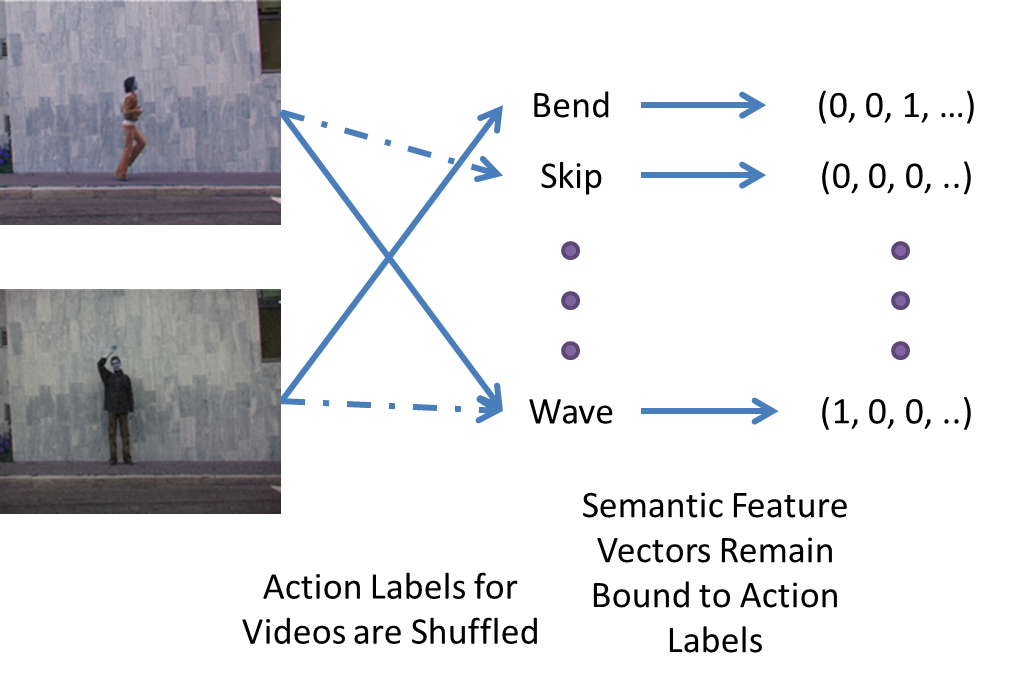
\includegraphics[width=.45\linewidth]{shuffle}
  \caption{Illustration of the permuting process. The action labels for each video in the training set were shuffled. Crucially, the action label semantic point representations were maintained so as to make a fair assessment.}
  \label{st}
\end{figure}

Performance of our two-stage algorithm in the leave-two-out cross-validation and rank experiments on this shuffled set approximates chance performance. Performance was measured for 250 trials in the leave-two-out cross-validation performance experiment, and 1000 in the rank experiment.
\label{stats}

\subsection{Materials}
\subsubsection{Data Sets}
Data was taken from the following two data sets: KTH \cite{kth} and Weizmann \cite{weizmann}. Both datasets contain videos for walking; these were combined and treated as a single class. The same applies to running.  When training and testing, however, we balanced the training set by ensuring that each action was represented by the same number of videos (10). Unfortunately, due to time constraints we were only able to randomize this balancing process for the leave-two-out cross-validation experiment (250 trials), and the permuted portion of the rank experiment (1000 trials). For the feature analysis experiments we worked with the complete set of videos (110).

\subsubsection{Semantic Features}
\label{sf}
The following are the semantic features that we selected, with values and explanations:
\begin{enumerate}
\item
$Coord\_arms$: Coordination of the arms. (Discrete 0-2) 0 is no coordination, 1 is coordination, 2 is anti-coordination.
\item
$Coord\_legs$: Coordination of the legs. (Discrete 0-2) 0 is none, 1 is coordination, 2 is anti-coordination.
\item
$Torso$: (Binary) 1 if torso is moving relative to the rest of the body.
\item
$Orient\_torso$: : (Discrete 0-2) 0 is that torso orientation is unrelated to the motion, 1 is that the torso is canonically parallel to motion, 2 is that the torso is canonically perpendicular to motion.
\item
$Vert$: (Discrete 0-5) amount of vertical displacement of the center of mass.
\item
$Horiz$: (Binary) 1 if there is whole body horizontal displacement.
\item
$Hand$: Hand location. (Binary) 1 if the hand is lower than the center of mass, 0 if it is higher.
\item
$Speed$: (Discrete 0-5) speed of center of mass.
\item
$Limbs$: (4 features, each Discrete 1-5) speed of each of the four limbs.
\end{enumerate}
\subsubsection{Coding Libraries}
This project was coded using Python. Basic libraries used include, SciPy \cite{scipy}, NumPy \cite{numpy}, OpenCV \cite{opencv}, and The Python Image Library \cite{pil}. Ridge regression and cross-validation code taken from Scikit-learn \cite{scikit}. Figures generated with MATLAB \cite{matlab}.

\section{Results}

\subsection{Leave-Two-Out Cross-Validation and Rank Performance}
Leave-two-out cross-validation performance was significantly above chance for most actions, as summarized in Figure \ref{ltocvplot}.  Performance averaged across actions was also statistically significant.

\begin{figure}[h]
  \centering
  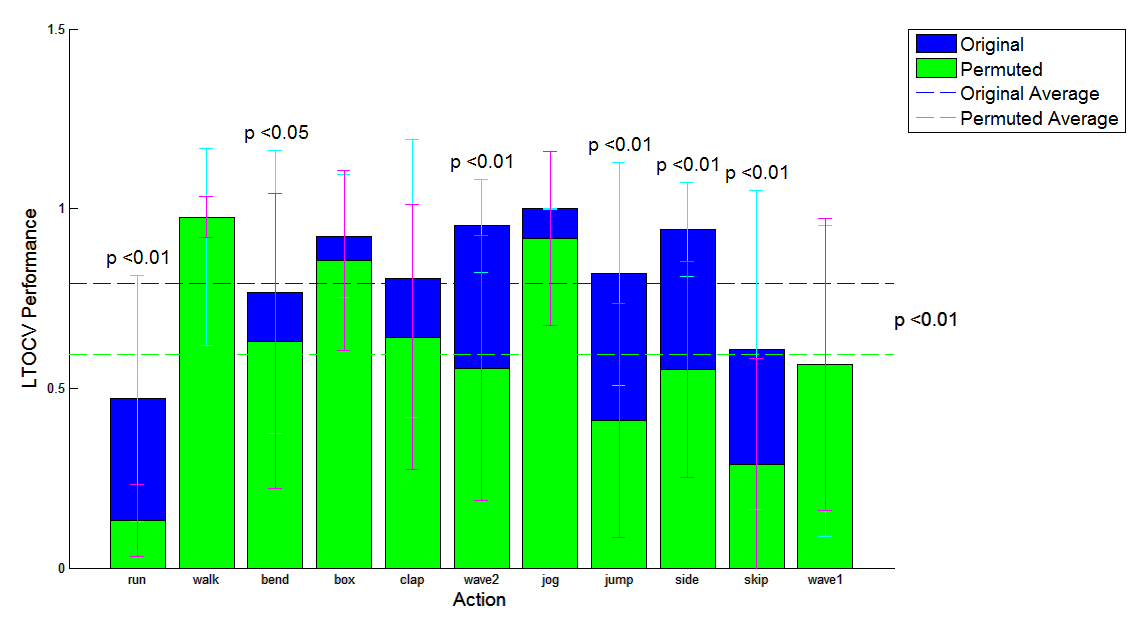
\includegraphics[width=.9\linewidth]{ltocv_snap_new}
  \caption{Results when comparing leave-two-out cross-validation (LTOCV) performance on the data set with labels intact (blue), and on the data set with labels permuted (green). Error bars are $\pm$ the standard deviation of the distribution of two vs two pairs.}
  \label{ltocvplot}
\end{figure}

Chance performance may seem high for two of the actions. This can be attributed to flaws in the semantic feature space, as there are some actions that, by nature of their location in the space, have a higher tendency to be selected.

Rank performance was also very significantly above chance for most actions, as well as for performance averaged across action. See Figure \ref{rankplot}. 

\begin{figure}[h]
  \centering
  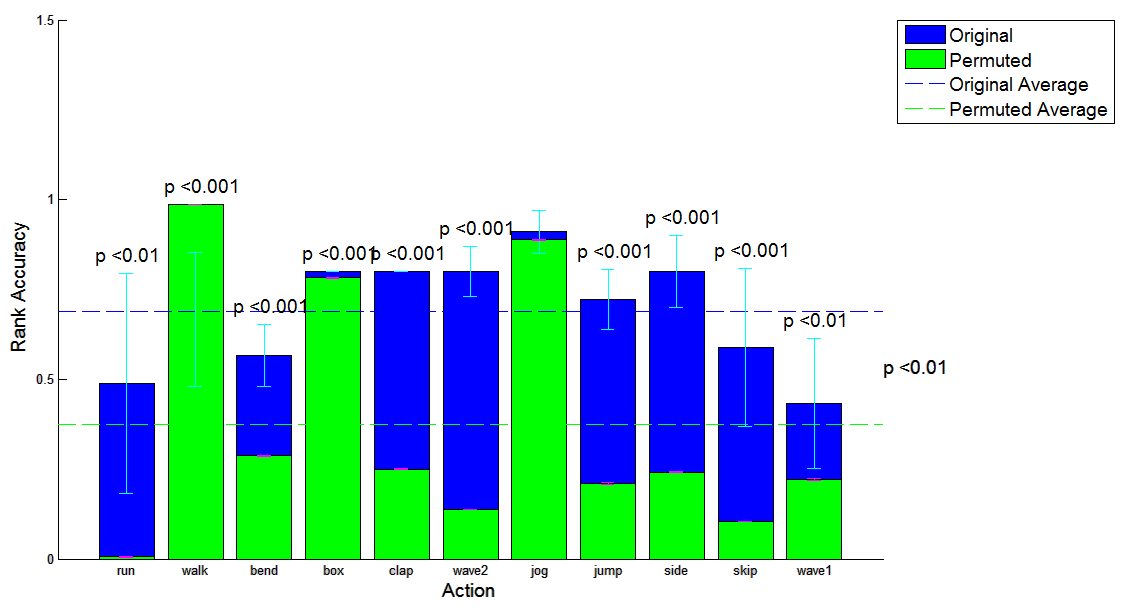
\includegraphics[width=.9\linewidth]{rank_snap_new}
  \caption{Rank test performance for the original (blue) and permuted (green) versions of the data set.  Error bars are $\pm$ the standard deviation of the distribution of rank scores for each video of a given action.}
  \label{rankplot}
\end{figure}

The variance of these results are noticeably lower than those of the leave-two-out cross-validation results, perhaps due to the nature of the score (there is a strict bound on the variance of a distribution of rank scores).  It also speaks to the consistency of the model that videos from the same action label tend to produce the same rank, even if that rank is not correct.

Unsurprisingly, actions that had high chance performance in leave-two-out cross-validation again had relatively high chance performance in this setting. An additional line of reasoning that can explain these results is the non-Euclidean nature of the semantic space. While using Euclidean distance clearly works reasonably well, more sophisticated notions of classification in this domain might yield better results in the form of greater difference between true and chance performance.

\subsection{Feature Comparison}

As is shown in Figure \ref{featplot}, no one feature is so important that its absence significantly affects performance, expecting the speed of the right arm.  However it is easy to see why, given that waving only involves that feature, it would hurt performance to not have it.

\begin{figure}[h]
  \centering
  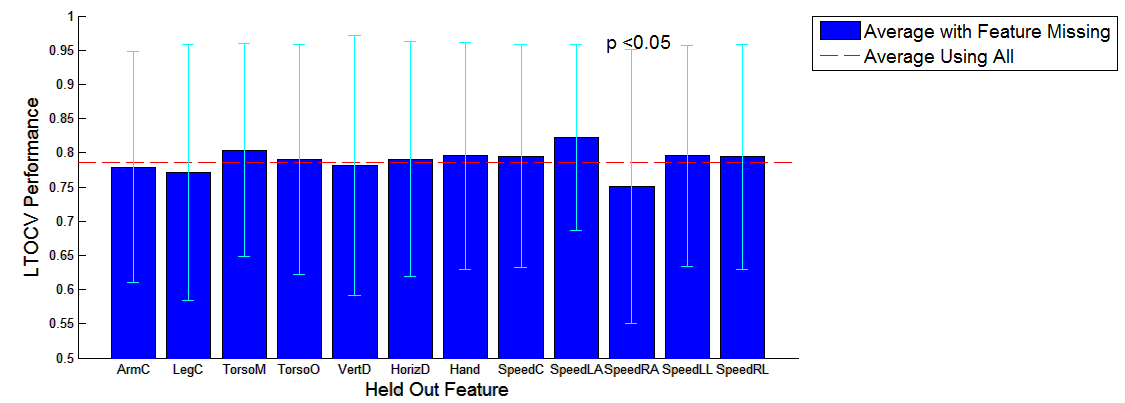
\includegraphics[width=.9\linewidth]{feature_snap}
  \caption{Performance of leave-two-out cross-validation versus held-out semantic feature. Average performance of the complete model is given by the dashed line. Error bars are $\pm$ standard deviation of the distribution over two vs two pairs.}
  \label{featplot}
\end{figure}

We also tried leaving out families of features, and the results are shown in Figure \ref{featgplot}.  This too did not affect performance significantly. It would appear that even removing highly correlated groups of features does not affect the classification results.

\begin{figure}[h]
  \centering
  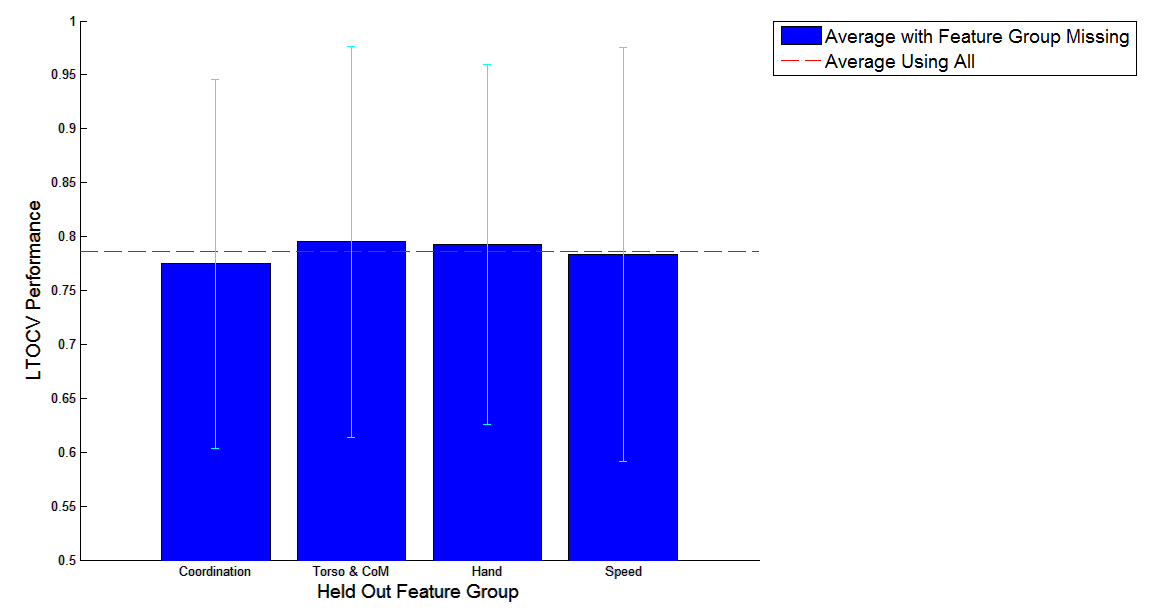
\includegraphics[width=.9\linewidth]{featuregrp_snap}
  \caption{Performance of leave-two-out cross-validation versus held-out semantic feature group (see Table \ref{featgrp}). Average performance of the complete model is given by the dashed line. Error bars are $\pm$ standard deviation of the distribution over two vs two pairs.}
  \label{featgplot}
\end{figure}

\section{Conclusion}
Our results demonstrate a proof-of-concept for zero shot learning in the domain of human action recognition from video. This technique allows extrapolation from labels in the training data set, so that we can classify videos with labels we have not yet seen.  Performance tended to vary depending on semantic feature and action, but was significantly better than noise in most cases. With a better-developed semantic feature base, we could see an improvement in results.

\bibliographystyle{ieeetr}
\bibliography{sources}

\end{document}
